\chapter{Variable Diffusivity}\label{ChapAppendVarDiff}
The resolution of the weather forecast (or reanalysis) data will not capture sub-grid
processes due to turbulent mixing in the atmosphere. To approximate this mixing, Ash3d
uses a diffusion term in the transport equation. A homogeneous and isotropic diffusivity
can be specified in the Ash3d control file, however it can be more realistic to 
treat the vertical and horizontal diffusivities separately and to have the values
depend on local atmospheric conditions.

The basic approach is to recognize that atmosphere is stratified and can be divided into
several layers within which the fundamental length-scale of turbulent mixing varies.
Broadly speaking, the atmosphere can be divided based on the temperature structure,
with the lowest level (the troposphere) consisting of a temperature profile that
decreases with altitude. This layer is characterized by strong vertical mixing and
contains the majority of the mass of the atmosphere and nearly all the atmospheric
water, essentially all the `weather'. This decrease in temperature with height is
interupted by the presence of ozone which reacts with solar radiation in a process that
releases heat, causing the temperature profile to increase with altitude. This layer
with the increase in temperature with height (stratosphere) is characterized by
minimal vertical mixing.
The change in lapse rate of the temperature defines the boundary between these layers
and is called the `tropopause'. Above the stratosphere, the temperature again decreases with
altitude in the mesosphere, then once again increases with height in the thermosphere
where incoming solar radiation once again plays a significant role.

For the purposes of volcanic ash transport modeling, we focus on the troposphere and
its sublayers as well as the stratosphere.
The primary layer of interest within the troposphere is the bottom layer
of the atmosphere where conditions are 
is effected by the surface. This layer is called the `atmospheric boundary layer' or
`planetary boundary layer' and is generally several hundred to a few thousand meters thick.
The thickness depends on several factors such as the latitude or the solar heating and
radiative cooling of the surface, as well as the temperature profile.
The bottom 10\% of this atmospheric boundary layer is called the `surface layer' and 
is generally well mixed, characterized by nearly homogeneous fluxes of heat and momentum.

Give description here of the diurnal nature of the atmospheric boundary layer, the surface
layer and the mixed layer with a figure modified after Stoll.

The approach we use in assigning a local diffusivity is by first identifying the location
of all these layers, then using the suitable expressions for calculating the local
diffusivity.

The primary driver of vertical mixing in the troposphere is the buoyant instability of a parcel
of air with respect to vertical perturbations in position. This can be quantified
by the dimensionless Richardson number, which is the ratio of the production of turbulent
kinetic energy via buoyancy to the production due to vertical shear stress.
The buoyant and shear stress terms can be approximated by vertical gradients of velocities
and virtual potential temperature and is given by
%% Richardson number (gradient) : Stull Eq. 5.6.2 or Monin and Yaglom Eq. 6.50 or Jacobson Eq 8.42
\begin{equation}\label{VarDiff_Eq_Rig}
\mathrm{Ri}_g = \frac{\frac{g}{\theta_v}\frac{\partial \theta_v}{\partial z}}
{\left( \frac{\partial u}{\partial z}\right)^2 + \left( \frac{\partial v}{\partial z}\right)^2}
\end{equation}
where $\theta_v$ is the virtual potential temperature and $u$ and $v$ are the horizontal velocities.

The virtual potential temperature is given by:
\begin{equation}\label{VarDiff_Eq_Thetav}
\theta_v = \theta \left[ 1 + \left( \frac{\mathrm{R}_{v}}{\mathrm{R}_{d}}-1\right) \, w_v \right] = \theta \left( 1 + 0.608 \, w_v \right)
\end{equation}
where $w_v$ is the mixing ratio of water vapor
(ratio of mass of water vapor to mass of dry air) % Stull 1.5.1b or Jacobson Eq 2.96
and $\mathrm{R}_{d}$ and $\mathrm{R}_{v}$ are the univerasal gas constants for dry air and vapor respectively.
The potential temperature $\theta$ is given by:
\begin{equation}\label{VarDiff_Eq_Theta}
\theta = T \left( \frac{p_0}{p}\right)^{\mathrm{R}_{d}/c_p} = T \left( \frac{p_0}{p}\right)^{0.286}
\end{equation}
where $p_0$ is the reference pressure (1000 $\mathrm{mb}$), and $c_p$ is the specific heat at constant pressure.
The vertical profile in potential temperature is useful in quickly determining if a region of the
atmosphere is stable or not depending on if the lapse rate is super- or sub-adiabatic.

The Richardson number also serves this purpose.
The denominator of $\mathrm{Ri}$ is strictly positive (turbulence by shear flow) whereas the numerator can be either
positive or negative depending the vertical gradient of $\theta_v$. For a dry, stable, vertically
stratified atmosphere, $\frac{\partial \theta}{\partial z}=0$.
If $\frac{\partial \theta_v}{\partial z}<0$ (i.e. $\mathrm{Ri}_g<0$), then there is a super-adiabatic lapse rate
and atmosphere is unstable with strong convection. In adiabatic conditions where
$\frac{\partial \theta_v}{\partial z} \rightarrow 0$ (and $\mathrm{Ri}_g \rightarrow 0$),
there is only mechanical turbulence. If $\frac{\partial \theta}{\partial z}>0$, then there
is a sub-adiabatic lapse rate and the mechanical production of turbulence is diminished by
the temperature stratification up until the Richardson number reaches a critical value,
$\mathrm{Ri} = \mathrm{Ri}_c$, above which all mechanical turbulence is suppressed.

Near the Earth's surface, the surface layer consists of the region in which turbulent fluxes,
both heat and stress, are roughly constant (vary by less than 10\%). Generally, with the constant
fluxes, variables in this surface layer can be characterized by a similarity solution as a function
of a few dimensionless groupings of variables. This Richardson number can be considered a dimensionless
length by defining:
\begin{equation}\label{VarDiff_Eq_ScaleHeight}
\mathrm{Ri} = \frac{z}{L}
\end{equation}
where $L$ is the Monin-Obukhov length which corresponds to the height where the buoyant energy production
equals the shear production. Because $\mathrm{Ri}$ can be either positive (stable) or negative (unstable), or
even 0 in perfectly neutral conditions where there is no buoyant turbulent energy production, $L$ is likewise
also either positive or negative, tending to $\infty$ in neutral conditions. 
The similarity variables proposed by Monin and Obukhov can be used to characterize an expression for 
a dimensionless velocity gradient.
\begin{equation}\label{VarDiff_Eq_Ugrad}
\phi(\zeta) = \frac{\kappa z}{u_*} \frac{\partial \overline{u_x}}{\partial z}  % S/P 16.37
\end{equation}
where $\zeta = z/L$.

To find $u$ as a function of height in the surface layer, $\frac{\partial \overline{u_x}}{\partial z}$
from Eq. \ref{VarDiff_Eq_Ugrad} can be integrated
which leads to a logarithmic velocity profile.
\begin{equation}\label{VarDiff_Eq_Ulog}
u(z) = \frac{u_{*}}{\kappa} \mathrm{ln} \frac{z-d}{z_0} + \psi (\zeta)
\end{equation}
where $d$ is the displacement height and $z_0$ is the aerodynamic roughness length. $\psi (\zeta)$ is
a function that results from integrating $\phi(\zeta)$.
$u_{*}$ is the friction velocity, which is a measure of the shear stress of the wind on the surface:
\begin{equation}\label{VarDiff_Eq_Ustar}
u_{*} = \sqrt{\frac{|\tau|}{\rho}}
\end{equation}

Note that the gradient Richardson number given above is an approximation to the flux
Richardson number which is given by
\begin{equation}\label{VarDiff_Eq_Rf}
\mathrm{Rf} = \frac{K_h}{K_m}\mathrm{Ri}_g
\end{equation}

Since $K_h \sim K_m$ in unstable conditions, we can alternatively express $L$ as
% Eq. 9.15 from Stull v2
\begin{equation}\label{VarDiff_Eq_Lalt}
L = -\frac{\rho c_p T_0 u^3_{*}}{\kappa g z \overline{q_z}} %Eq 16.70 S/P
\end{equation}


%%%%%%%%%%%%%%%%%%%%%%%%%%%%%%%%%%%%%%%%%%%%%%%%%%%%%%%%%%%%%%%%%%%%%%%%%%%%%%%
%%%%%%%%%%%%%%%%%%%%%%%%%%%%%%%%%%%%%%%%%%%%%%%%%%%%%%%%%%%%%%%%%%%%%%%%%%%%%%%
%%%%%%%%%%%%%%%%%%%%%%%%%%%%%%%%%%%%%%%%%%%%%%%%%%%%%%%%%%%%%%%%%%%%%%%%%%%%%%%

\section{Atmospheric stability metrics and layer boundaries}
%%%%%%%%%%%%%%%%%%%%%%%%%%%%%%%%%%%%%%%%%%%%%%%%%%%%%%%%%%%%%%%%%%%%%%%%%%%%%%%
\subsection{Richardson number}

In Ash3d, $\mathrm{Ri}_g$ is approximated with the bulk Richardson number, which
only requires values at discrete levels.
% Richardson number (bulk) : Stull Eq. 5.6.3 or Jacobson Eq 8.39
\begin{equation}\label{VarDiff_Eq_Rib}
\mathrm{Ri}_b = \frac{g \Delta \theta_v \Delta z}
{\theta_v \left[ \left( \Delta u \right)^2 + \left( \Delta v \right)^2 \right]}
\end{equation}

The virtual potential temperature, $\theta_v$ requires the water mixing ratio, $w_v$,
through Eq. \ref{VarDiff_Eq_Thetav}. Generally, this is not provided
in the NWP files, but can be related to the specific humidity, $q$, through the relation
$w_v=q/(1-q)$

%If \texttt{useMoisture=.true.} in the Variable Diffusivity input block, then Ash3d will attempt to
%read liquid water mixing ratios from the provided NWP file.
%If $w_v$ is not available but specific humidity ($q$) is, $w_v$ will be calculated from $q$ (ratio of mass of
%water vapor to total mass of air) via the relation $w_v=q/(1-q)$.
If neither $q$ nor $w_v$ is available or if \texttt{useMoisture=.false.}, then
the virtual potential temperature will be replaced by the potential temperature in Eq. \ref{VarDiff_Eq_Rib}.
$q$ typically does not exceed $0.02 \, \mathrm{kg}/\mathrm{kg}$ so the difference between $\theta_v$
and $\theta$ is generally less than 1\%.

%%%%%%%%%%%%%%%%%%%%%%%%%%%%%%%%%%%%%%%%%%%%%%%%%%%%%%%%%%%%%%%%%%%%%%%%%%%%%%%
\subsection{Monin-Obukhov Length}
From Eq. \ref{VarDiff_Eq_ScaleHeight}, the Monin-Obukhov length can be expressed as
a simple function of $z$ and $\mathrm{Ri}$, but empirical studies found that
the expression for $L$ should be separated into one for unstable and one for stable 
atmospheric conditions.
\begin{eqnarray}\label{VarDiff_Eq_MonL}
L &=& \left\{ \begin{array} {l@{\quad \quad}l}
 \frac{z}{\mathrm{Ri}}                 &:  \mathrm{if}\,\,\, \mathrm{Ri}<0 \,\,\, \mathrm{unstable} \\
\frac{z}{\mathrm{Ri}}\left(1-5\,\mathrm{Ri}\right)  &:  \mathrm{if}\,\,\, \mathrm{Ri}>0 \,\,\, \mathrm{stable}
\end{array}
\right.
\end{eqnarray}


%%%%%%%%%%%%%%%%%%%%%%%%%%%%%%%%%%%%%%%%%%%%%%%%%%%%%%%%%%%%%%%%%%%%%%%%%%%%%%%
\subsection{Friction Velocity}
The friction velocity, $u_*$, is a characteristic velocity important in building a similarity
solution in the surface layer. Though it has units of velocity, it is really a measure
of the magnitude of the Reynolds shear stress on the surface given in Eq. \ref{VarDiff_Eq_Ustar}.
In Ash3d, $u_*$ is first attempted to be directly loaded from the NWP file. If this variable is not
provided by the forecast/reanalysis data, then $u_*$ is calculated from evaluating the velocity
profile (Eq. \ref{VarDiff_Eq_Ulog}) at a reference height, $z_r$.
\begin{equation}\label{VarDiff_Eq_Ustar2}
u_* = \frac{\kappa |u(z_r)|}{\ln \frac{z_r-d}{z_0} - \psi(\frac{z_r}{L})}
\end{equation}
Equation \ref{VarDiff_Eq_Ustar2} is only valid in the surface layer, within which
$u_*$ and $L$ are constant for any pairing of $z_r$ and $u(z_r)$. If $u_*$ is not directly available
from the NWP data, Ash3d attempts to read $u$ and $v$ at either then 2 or 10 meter levels then to
use in Eq. \ref{VarDiff_Eq_Ustar2}. If these are also not provided, $u$ and $v$ from the largest
pressure level are used.


%%%%%%%%%%%%%%%%%%%%%%%%%%%%%%%%%%%%%%%%%%%%%%%%%%%%%%%%%%%%%%%%%%%%%%%%%%%%%%%
\subsection{Atmospheric boundary layer height}

There are many methods to determine or approximate the height of the atmospheric boundary
layer (ABL), several of which are described in \ref{Sugiyama99}. One method relies only on the
vertical temperature gradient, noting that temperature inversions in the lower troposphere
are likely the capping inversions often observed at the ABL. This
approach from \ref{Heffter80} identifies the lowest point in which the lapse rate
\begin{equation}\label{VarDiff_Eq_ABL1}
\frac{\Delta \theta}{\Delta z} \ge 0.005 \, \mathrm{K} / \mathrm{m}
\end{equation}
and the temperature difference between the inversion base and top
is $\Delta \theta > 2 \, \mathrm{K}$.

If there is no capping inversion layer resolved by the NWP data, then this method
will flag the tropopause as the ABL height.

An alternative method is to use the thickness of the Ekman layer as the ABL height.
This method works for neutral or stable atmospheric conditions. The Ekman layer is
controlled in part by the Coriolis paramter, $f=2 \Omega \sin \phi$ where $\phi$
is the latitude and $\Omega$ is the rotation rate of the Earth
($7.292 \times 10^{-5} \, \mathrm{rad/s}$).  For neutral conditions,
when $\left| \frac{u_*}{f L}\right| < 4$, the ABL height is given by
\begin{equation}\label{VarDiff_Eq_ABL2_1}
h_{ABL} = \frac{c_n u_*}{|f|}
\end{equation}
Eq. \ref{VarDiff_Eq_ABL2_1} becomes singular with $\phi \rightarrow 0$, so a minumum
of $\phi=20^{\circ}$ is used. $c_n$ can be from 0.07 to 0.5, but we use $c_n=0.2$.

For stable conditions, where $\left| \frac{u_*}{f L}\right| \ge 4$, the ABL height is given by
\begin{equation}\label{VarDiff_Eq_ABL2_2}
h_{ABL} = c_s \sqrt{\frac{u_* L}{|f|}}
\end{equation}
where $c_s=0.4$.

Finally, a third approach uses the bulk Richardson number. The ABL height is identified as the
lowest point where the Richardson number exceeds a threshold value, typically $\mathrm{Ri}_c=$ 0.25 or
0.5.




%%%%%%%%%%%%%%%%%%%%%%%%%%%%%%%%%%%%%%%%%%%%%%%%%%%%%%%%%%%%%%%%%%%%%%%%%%%%%%%
\subsection{Tropopause}
To determine the height of the tropopause, Ash3d calculates the lapse rate,
$\Gamma = -\partial T/\partial z$, and searches for the location of $\Gamma<0$.
Since there are occasional temperature inversion layers in the lower troposphere
that cap the atmospheric boundary layer,
the lowest point greater then 5 $\mathrm{km}$ with $\Gamma<0$ is marked as the
height of the tropopause.




%The basic
%structure of the block consists of three input lines:
%\small
%\begin{verbatim}
%yes 1                       # use horizontal variable diffusivity; model ID
%yes                         # use vertical variable diffusivity
%0.9                         # KH_SmagC
%0.4                         # vonKarman
%30.0                        # LambdaC
%0.25                        # RI_CRIT
%\end{verbatim}
%\normalsize

%%%%%%%%%%%%%%%%%%%%%%%%%%%%%%%%%%%%%%%%%%%%%%%%%%%%%%%%%%%%%%%%%%%%%%%%%%%%%%%
%%%%%%%%%%%%%%%%%%%%%%%%%%%%%%%%%%%%%%%%%%%%%%%%%%%%%%%%%%%%%%%%%%%%%%%%%%%%%%%
%%%%%%%%%%%%%%%%%%%%%%%%%%%%%%%%%%%%%%%%%%%%%%%%%%%%%%%%%%%%%%%%%%%%%%%%%%%%%%%
\section{Local Diffusivity}
\subsection{Horizontal Diffusivity}\label{ChapAppendVarDiff_Sec_Kh}
For deteriming the horizonal diffusivity, Ash3d uses the Smagorinski model which
applies a diffusivity to account for the turbulent fluctuations that are smaller
than the model grid. The diffusivity is related to the vertical gradients in
horizontal velocities and the cell-size of the velocity model.

\begin{equation}\label{VarDiff_Eq_Smag}
K_h = C \Delta x \Delta y \sqrt{\left[ \frac{\partial u}{\partial x} -\frac{\partial v}{\partial y} \right]^2
+ \left[ \frac{\partial v}{\partial x} +\frac{\partial u}{\partial y} \right]^2}
\end{equation}

The first term in the radical is the ``horizontal tension'' term and the second is
the ``horizontal shearing strain'' term \cite{Griffies2000}.
As a whole, the radical has units of $\mathrm{t}^{-1}$.
The length scale should be proportional to the maximum wavenumber represented by the grid.
Since this is determined by the grid of the NWP data, the $\Delta x$ and $\Delta y$ are the 
corresponding horizontal length scales of the NWP data. Ash3d used the area of the cells
for this product. $C$ is a dimensionless scaling parameter.

An alternate model which uses a slightly different ``tension'' term is the Pielke model.
\begin{equation}\label{VarDiff_Eq_Pielke}
K_h = C \Delta x \Delta y \sqrt{
\frac{1}{2}\left[ \left(\frac{\partial u}{\partial x}\right)^2 + \left(\frac{\partial v}{\partial y}\right)^2 \right]
+ \left[ \frac{\partial v}{\partial x} +\frac{\partial u}{\partial y} \right]^2}
\end{equation}


%%%%%%%%%%%%%%%%%%%%%%%%%%%%%%%%%%%%%%%%%%%%%%%%%%%%%%%%%%%%%%%%%%%%%%%%%%%%%%%
%%%%%%%%%%%%%%%%%%%%%%%%%%%%%%%%%%%%%%%%%%%%%%%%%%%%%%%%%%%%%%%%%%%%%%%%%%%%%%%
%%%%%%%%%%%%%%%%%%%%%%%%%%%%%%%%%%%%%%%%%%%%%%%%%%%%%%%%%%%%%%%%%%%%%%%%%%%%%%%
\section{Vertical Diffusivity}\label{ChapAppendVarDiff_Sec_Kv}
The formulation for vertical diffusivity depends on which region of the atmosphere
we are considering, primarily whether the point is within the atmospheric boundary
layer (and more specifically, in either the surface layer or the mixed layer),
or in the free atmosphere above the boundary layer.

%%%%%%%%%%%%%%%%%%%%%%%%%%%%%%%%%%%%%%%%%%%%%%%%%%%%%%%%%%%%%%%%%%%%%%%%%%%%%%%
\subsection{Free Atmosphere}
In the region of the atmosphere above the boundary layer, the formulation of diffusivity
from Prantl (1932) relates $K_z$ to shear stresses using the vertical gradient in
horizontal velocity through a mixing length, $\ell_m$. % Randerson %Eq.5.23, Monin 5.112,Stull 6.4.4f
Typically, this is scaled by a non-dimensional stability function of $\mathrm{Ri}$ so as to
include the effects of buoyancy.
% Jacobson Eq.8.70
\begin{equation}\label{VarDiff_Eq_Kz_FreAtmos}
K_z = \ell_m^2 \frac{\partial \overline{u}}{\partial z}  \mathcal{F}(\mathrm{Ri})
\end{equation}
where the mixing length, $\ell_m$ follows the relation
\begin{equation}\label{VarDiff_Eq_MixLen}
\frac{1}{\ell_m} = \frac{1}{\kappa z} + \frac{1}{\lambda_m}
\end{equation}

%\begin{equation}
%\ell_m = \frac{\kappa z}{1+ \frac{\kappa z}{\lambda_m}}
%\end{equation}
For stable or weakly unstable conditions, the stability function can be expressed as
$\mathcal{F}(\mathrm{Ri}) = (\mathrm{Ri}_c-\mathrm{Ri})/\mathrm{Ri}$ \cite{Jacobson2005}, %Jacobson Eq.8.70
but this breaks down as $\mathrm{Ri}$ becomes more negative. In these situations, vertical mixing
is dominated by free convection and the vertical diffusivity model does not apply.

Alternatively, Collins et al \ref{Collin} use the following form for the stability function.
\begin{eqnarray}\label{VarDiff_Eq_F_Collins}
\mathcal{F}(\mathrm{Ri}) &=& \left\{ \begin{array} {l@{\quad \quad}l}
 \left[ 1 -18 \, \mathrm{Ri} \right]^{1/2}                         &: \mathrm{if}\,\,\, \mathrm{Ri} < 0 \,\,\, \mathrm{unstable} \\
 \left[ 1+ 10 \, \mathrm{Ri} \, (1+8 \, \mathrm{Ri}) \right]^{-1}  &: \mathrm{if}\,\,\, \mathrm{Ri} > 0 \,\,\, \mathrm{unstable}
\end{array}
\right.
\end{eqnarray}


\begin{figure}[htbp]\vspace*{0cm}\hspace*{0cm}
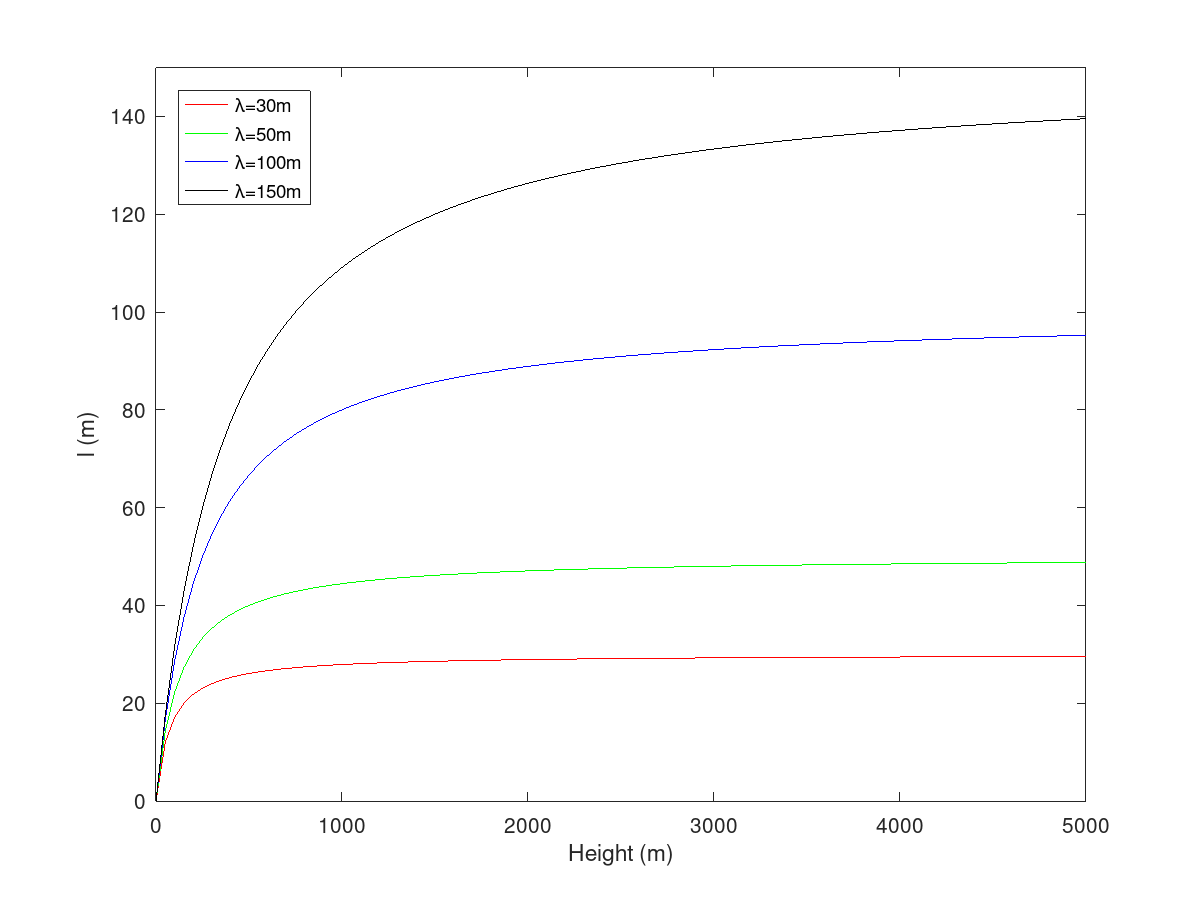
\includegraphics[angle=0,scale=0.2]{Figures/Apx_VarDiff/Kz_MixLen.png}
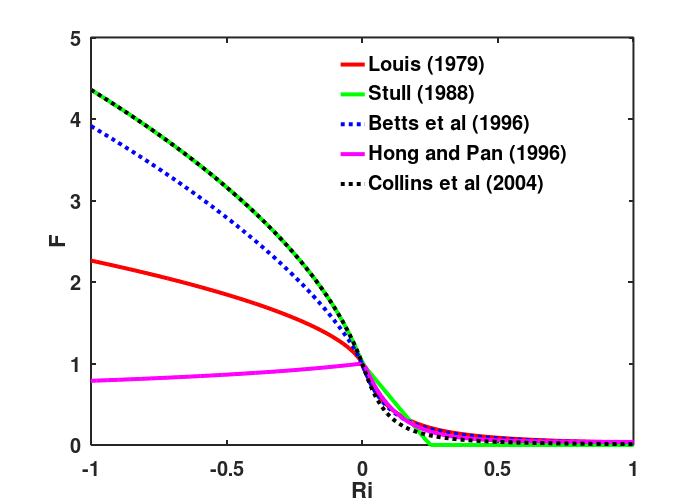
\includegraphics[angle=0,scale=0.2]{Figures/Apx_VarDiff/Kz_Fc.png}\\
\parbox{15cm}{\caption{\label{FigVarDiff_Kz_MixLen}
Mixing Length
}}
\end{figure}


%%%%%%%%%%%%%%%%%%%%%%%%%%%%%%%%%%%%%%%%%%%%%%%%%%%%%%%%%%%%%%%%%%%%%%%%%%%%%%%
\subsection{Surface Layer}

The Monin-Obukhov similarity description of the surface layer leads to the following
expression for the vertical diffusivity.
\begin{equation}\label{VarDiff_Eq_Kz_Surf}
K_v = \frac{u_{*} \kappa z}{\phi(\zeta)}
\end{equation}
where the term $\kappa z / \phi(\zeta)$ is effectively the mixing length as a function of height from the
surface. $\phi(\zeta)$ is the dimensionless velocity gradient 
function from Eq. \ref{VarDiff_Eq_Ugrad} which is unity for neutral conditions ($\zeta=0$),
$\phi(\zeta)>1$ for stable conditions ($\zeta>0$) and $\phi(\zeta)<0$ for unstable
conditions $\phi(\zeta)<0$.
Note that this term is essentially $\ell_m$ from Eq. \ref{VarDiff_Eq_MixLen} in the limit of
$\kappa z << \lambda_m$ for neutral conditions. $\phi(\zeta)$ is strictly positive and
has the effect of scaling the growth of the mixing length, either minimizing it in
stable conditions, or magnifying it in unstable conditions. In neutral conditions, the
mixing length (and $K_v$) grows proportional to the distance from the surface within the
surface layer. 

Several expressions for $\phi(\zeta)$ have been suggested by various authors with a
general form given below.

\begin{eqnarray}\label{VarDiff_Eq_PhiB}
\phi &=& \left\{ \begin{array} {l@{\quad \quad}l}
 \left[ 1+\gamma \zeta\right]^{\alpha}  &:  \mathrm{if}\,\,\, \zeta < 0 \,\,\, \mathrm{unstable} \\
1                                       &:  \mathrm{if}\,\,\, \zeta = 0 \,\,\, \mathrm{neutral} \\
1 + \beta \zeta                         &:  \mathrm{if}\,\,\, \zeta > 0 \,\,\, \mathrm{stable}
\end{array}
\right.
\end{eqnarray}

Frequently used values are given below.
\small
\begin{table}[htbp]
\begin{center}
\begin{tabular}{| c | c | c | c |}
\hline
Author & $\alpha$ & $\beta$ & $\gamma$\\
\hline
Businger-Dyer (1971)     & -1/4 & 5.0 & -16.0 \\
Carl (1973)              & -1/3 & 5.0 & -15.0 \\
\hline
\end{tabular}
\caption{\label{Tab_VarDiff_phisurf}Coefficients for $\phi$ in the surface layer}
\end{center}
\end{table}
\normalsize

Panofsky reports that an exponent $\alpha=-1/3$ is theoretically preferable
since $\phi$ follows $(z/L)^{-1/3}$ for large $-z/L$ (free-convection condition) Pan. p134.
$\beta$ should be from 4.7 to 5.2 (Pan. p136.).

%%%%%%%%%%%%%%%%%%%%%%%%%%%%%%%%%%%%%%%%%%%%%%%%%%%%%%%%%%%%%%%%%%%%%%%%%%%%%%%
\subsection{Mixed Layer}
In the mixed layer above the surface layer, but below the atmospheric boundary layer,
the logarithmic velocity profile as well as all other implications of the similarity
solution break down. To extend $K_v$ above the surface layer, a few modifications to
Eq. \ref{VarDiff_Eq_PhiB} have been proposed to scale back the increase in $K_v$ with
height to match the free-atmosphere conditions above the ABL.

For neutral and stable conditions, one method is the use a decaying exponential scale
factor.
\begin{equation}\label{VarDiff_Eq_Kz_Mixed_Exp}
K_z = \frac{u_{*} \kappa z}{\phi} \exp \left( -\frac{8 f z}{u_*} \right)
\end{equation}
In this equation, $f$ is the Coriolis parameter described above and $f/u_*$ is
the Ekman layer height. This formula can be used for all heights as the exponential
term ensures that $K_z$ from the surface layer approximation becomes vanishingly
small above the ABL.

An alternative formulation is to scale Eq. \ref{VarDiff_Eq_PhiB} by a polynomial taper
up to the ABL.
\begin{equation}\label{VarDiff_Eq_Kz_Mixed_Poly}
K_z = \frac{u_{*} \kappa z}{\phi} \left( 1-\frac{z}{h_{BL}} \right)^p
\end{equation}
This equation is not valid above the ABL.

In both forms above, the general expression for $\phi(\zeta)$ given in Eq. \ref{VarDiff_Eq_PhiB}
can be used, but the coefficients should be modified to account for the deviation in the
surface layer due to the scaling term.

\small
\begin{table}[htbp]
\begin{center}
\begin{tabular}{| c | c | c | c | c |}
\hline
Author & $\alpha$ & $\beta$ & $\gamma$ & p \\
\hline
Businger-Dyer (1971)     & -1/4 & 5.0 & -16.0 & N/A \\
Troen-Mahrt (1986) \cite{Troen1986}      & -1/3 & 5.0 & -7.0  & 2 \\
Ulke (2000)        \cite{Ulke2000}      & -1/2 & 9.2 & -13.0 & 1 \\
\hline
\end{tabular}
\caption{\label{tab:ProjOpt}Ash3d projection options}
\end{center}
\end{table}
\normalsize



